\section{Transport-Gleichungen} \marginpar{VL 27}
\begin{itemize}
    \item[] bisher: Gleichgewicht $\widehat{=}$ \say{Thermostatistik}
    \item[] jetzt: Nicht-Gleichgewicht: Dynamik, Transport, Weg ins Gleichgewicht
\end{itemize}

\subsection{Boltzmann-Gleichung, H-Theorem}
\subsubsection*{Boltzmann-Gleichung}
verdünntes Gas mit $\lambda \ll \left(\frac{V}{N}\right)^{1/3} \quad \Rightarrow$ klassische Beschreibung

\paragraph{bisher:}
\begin{itemize}
    \item[] N-Teilchen Phasenraum: $(q_1,...,q_f,p_1,...,p_f) \qquad f= 3N$
    \item[] Mikrozustand: Punkt im 6N-dimensionalen Phasenraum
    \item[] Makrozustan: WS-Dichte $\varrho(q_1,...,q_f,p_1,...,p_f)$
\end{itemize}

\paragraph{jetzt:}
\begin{itemize}
    \item[] Einteilchen-Phasenraum $\Vec{q}, \Vec{p}$ mit f = 6
    \item[] Mikrozustand: N Punkte im Einteilchen-Phasenraum
    \item[] $\stackrel{\text{nähern}}{\longrightarrow}$ WS-Dichte $f(\Vec{q},\Vec{p},t)$ mit
    \begin{equation}
        f(\Vec{q},\Vec{p},t) \cdot d^3q \ d^3p \qq{Zahl der Teilchen im Volumen} d^3q \ d^3p
    \end{equation}
    \item[$\Rightarrow$] $\int \ f(\Vec{q},\Vec{p},t) \ d^3q d^3p \ = \ N$  
\end{itemize}

\paragraph{Ziel:} Bestimme $f(\Vec{q},\Vec{p},t)$ in Abhängigkeit von WW zwischen den Teilchen. \color{black!40} (deutlich einfacher als 6N-dim. Phasenraum, aber nicht vollst. Information; Reduktion bis auf 1D möglich) \color{black}

\paragraph{ohne WW:}
Hamilton-Bewegungsgleichung:
\begin{equation}
    \dot{\Vec{q}} = \pdv{H}{\Vec{p}} = \frac{\Vec{p}}{m} \qquad \dot{\Vec{p}} = - \pdv{H}{\Vec{q}} = \Vec{F} \qq{\color{black!40}(Kraft)\color{black}}
\end{equation}
Liouville-Theorme:
\begin{align}
    0 = \dv{f(\Vec{q},\Vec{p},t)}{t} &= \pdv{f}{t} + \pdv{f}{\Vec{q}} \Dot{\Vec{q}} + \pdv{f}{\Vec{p}} \Dot{\Vec{p}} \\
    &\Longrightarrow \left( \pdv{}{t} + \frac{\Vec{p}}{m} \pdv{}{\Vec{q}} + \Vec{F} \pdv{}{\Vec{p}} \right) f(\Vec{q},\Vec{p},t) = 0 \qq{stoßfreie Boltzmann-GL}
\end{align}
Sei:
\begin{itemize}
    \item $\Vec{F}=0$
    \item homogen im Ort $\Rightarrow \ f(\Vec{p},t)$
    \item[] $\Rightarrow \quad \pdv{f(\Vec{p},t)}{t}=0$
    \item[] $\Rightarrow$ jede zeitlich konstante Wahscheinlichkeitsdichte $f(\Vec{p})$ ist Lösung
    \item[] $\Rightarrow$ kein Weg ins GG ohne WW
\end{itemize}

\subsubsection*{mit WW:}
\begin{definition}{Boltzmann-Gleichung}
    \begin{equation}
    \left( \pdv{}{t} + \frac{\Vec{p}}{m} \pdv{}{\Vec{q}} + \Vec{F} \pdv{}{\Vec{p}} \right) f(\Vec{q},\Vec{p},t) = \left(\pdv{f(\Vec{q},\Vec{p},t)}{t}\right)_{\text{Stöße}}
    \end{equation}
\end{definition}

verdünntes Gas $\Rightarrow$ Stoßdauer $\ll$ Zeit zwischen Stößen $\Rightarrow$ nur 2-Teilchen-Stöße wichtig
\begin{figure}[h]
    \centering
    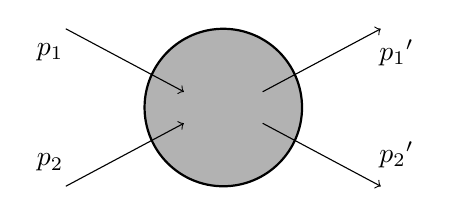
\begin{tikzpicture}
        \filldraw[fill=black!30, draw=black,thick] (0,0) circle (1);
        \draw[->] (-2,1) -- (-0.5,0.2);
        \draw (-2.2,0.7) node{$\Vec{p_1}$};
        \draw[->] (-2,-1) -- (-0.5,-0.2);
        \draw (-2.2,-0.7) node{$\Vec{p_2}$};
        \draw[->] (0.5,0.2) -- (2,1);
        \draw (2.2,0.7) node{$\Vec{p_1}^\prime$};
        \draw[->] (0.5,-0.2) -- (2,-1);
        \draw (2.2,-0.6) node{$\Vec{p_2}^\prime$};
    \end{tikzpicture}
\end{figure}

Zahl der Stoßpaare $\Vec{p}_1,\Vec{p}_2$ bei $\Vec{q}$:
\begin{align}
    dN = \underbrace{F(\Vec{q},\Vec{p}_1,\Vec{p}_2,t)}_{\substack{\text{2-Teilchen-Korrelationen,}\\ \text{unbekannt}}}\ d^3q \ d^3p_1 \ d^3p_2 \\
    \Rightarrow \quad \left(\pdv{f(\Vec{q},\Vec{p},t)}{t}\right)_{\text{Stöße}} = \int &\ d^3p_2 \ d^3p_1^\prime \ d^3p_1^\prime \cdot \underbrace{\delta^3(\Vec{p_1}^\prime + \Vec{p_2}^\prime - (\Vec{p}_1 + \Vec{p}_2)) }_{\text{Impulserhaltung}}\\
    &\cdot \underbrace{\delta\left(\frac{\abs{\Vec{p}_1^\prime}^2}{2m} + \frac{\abs{\Vec{p}_2^\prime}^2}{2m} - \left(\frac{\abs{\Vec{p}_1}^2}{2m} + \frac{\abs{\Vec{p}_2}^2}{2m}\right)\right)}_{\text{Energieerhaltung}} \\
    &\cdot \underbrace{\abs{T_{12\rightarrow1^\prime2^\prime}}^2}_{\text{qm. Streumatrixelement}} \\
    &\cdot \underbrace{\left(F(\Vec{q},\Vec{p}_1^\prime,\Vec{p}_2^\prime,t) - F(\Vec{q},\Vec{p}_1,\Vec{p}_2,t) \right)}_{\text{Zeitumkehr} \; (T_{12\rightarrow1^\prime2^\prime} = T_{1^\prime2^\prime\rightarrow12})}
\end{align}

Stoßzahlansatz (d.h. unkorrelierte Impulse):
\begin{align}
    F(\Vec{q},\Vec{p}_1,\Vec{p}_2,t) = \underbrace{f(\Vec{q},\Vec{p}_1,t)}_{=: f_1} &\cdot \underbrace{f(\Vec{q},\Vec{p}_2,t)}_{=: f_2} \\ \label{eq.Boltzmann}
    \left( \pdv{}{t} + \frac{\Vec{p}}{m} \pdv{}{\Vec{q}} + \Vec{F} \pdv{}{\Vec{p}} \right) f(\Vec{q},\Vec{p}_1,t) = \int &\ d^3p_2 \ d^3p_1^\prime \ d^3p_1^\prime \cdot \delta^3(\Vec{p}_f-\Vec{p}_i) \cdot \delta(E_f-E_i) \\
    &\cdot \abs{T_{i\rightarrow f}}^2 \cdot \left(f_1^\prime \cdot f_2^\prime -f_1\cdot f_2 \right)
\end{align}

\subsubsection*{H-Theorem}
Sei:
\begin{itemize}
    \item $\Vec{F}=0$
    \item homogen im Ort: $f=f(\Vec{p},t)$
    \item[$\Rightarrow$] linke Seite in \cref{eq.Boltzmann} nur $\pdv{}{t} f(\Vec{p}_1,t)$
\end{itemize}
Definiere nun (verwandt mit Entropie):
\begin{align}
    H(t) := \int \ d^3p_1 \ f(\Vec{p_1},t) \ \ln(f(\Vec{p}_1,t))
\end{align}

\begin{definition}{Boltzmann H-Theorem}
    \begin{equation}
        \dv{H(t)}{t} \leq 0
    \end{equation}
\end{definition}

\begin{proof}
\begin{align}\label{5_ableitung1}
    \dv{H}{t}&= \int \ d^3p_1 \ \pdv{f(\Vec{p_1},t)}{t} \left( \ln(f(\Vec{p}_1,t)) + 1\right)\\
    &= \int \ d^3p_1 \ d^3p_2 \ d^3p_1^\prime \ d^3p_2^\prime \ \delta^3(\Vec{p}_f-\Vec{p}_i)\cdot \delta(E_f-E_i)\cdot \abs{T_{i\rightarrow f}}^2 \\
    &\qquad \cdot (f_1^\prime f_2^\prime-f_1 f_2)\cdot (1+\ln(f(\Vec{p}_1,t)))
\end{align}
vertausche $\Vec{p}_1, \ \Vec{p}_2$:
\begin{align}\label{5_ableitung2}
    \dv{H}{t} = \int \ d^3p_1 \ d^3p_2 \ d^3p_1^\prime \ d^3p_2^\prime \ \delta^3(\Vec{p}_f-\Vec{p}_i)\cdot \delta(E_f-E_i)\cdot \abs{T_{i\rightarrow f}}^2 \\
    \qquad \cdot (f_1^\prime f_2^\prime-f_1 f_2)\cdot (1+\ln(f(\Vec{p}_2,t)))
\end{align}
addiere \cref{5_ableitung1} und \cref{5_ableitung2} und dividiere durch 2:
\begin{align}\label{5_ergebnis1}
    \dv{H}{t} = \int \ d^3p_1 \ d^3p_2 \ d^3p_1^\prime \ d^3p_2^\prime \ \delta^3(\Vec{p}_f-\Vec{p}_i)\cdot \delta(E_f-E_i)\cdot \abs{T_{i\rightarrow f}}^2 \\
    \qquad \cdot (f_1^\prime f_2^\prime-f_1 f_2)\cdot \frac{1}{2} \cdot (2+\ln(f_1f_2))
\end{align}
vertausche $\Vec{p}_1, \ \Vec{p}_2$ mit $\Vec{p}_1^\prime, \ \Vec{p}_2^\prime$:
\begin{align}\label{5_ableitung3}
    \dv{H}{t} = \int \ d^3p_1 \ d^3p_2 \ d^3p_1^\prime \ d^3p_2^\prime \ \delta^3(\Vec{p}_f-\Vec{p}_i)\cdot \delta(E_f-E_i)\cdot \abs{T_{i\rightarrow f}}^2 \\
    \qquad \cdot (f_1^\prime f_2^\prime-f_1 f_2)\cdot \frac{1}{2} \cdot (2+\ln(f_1^\prime f_2^\prime))
\end{align}
addiere \cref{5_ableitung3} zu \cref{5_ergebnis1}:
\begin{align}
    \Longrightarrow \ \dv{H}{t} = \frac{1}{4}\cdot \int \ d^3p_1 \ d^3p_2 \ d^3p_1^\prime \ d^3p_2^\prime \ \delta^3(\Vec{p}_f-\Vec{p}_i)\cdot \delta(E_f-E_i)\cdot \abs{T_{i\rightarrow f}}^2 \\
    \qquad \cdot \underbrace{(f_1^\prime f_2^\prime-f_1 f_2)}_{=: y-x} \cdot \underbrace{(\ln(f_1 f_2)+\ln(f_1^\prime f_2^\prime))}_{=: \ln x -\ln y}
\end{align}
nutze $(y-x)\cdot (\ln x -\ln y) \leq 0$ mit \say{=} falls $x=y$
\begin{equation}
    \Longrightarrow \; \dv{H}{t} \leq 0
\end{equation}
\end{proof}

\paragraph{Bemerkung:}
\begin{equation}
    \Dot{\Tilde{S}} = -k \cdot \Dot{H} \geq 0 \qq{Entropie wächst}
\end{equation}
\begin{itemize}
    \item ausgezeichnete Zeitrichtung
    \item Grund: Stoßzahlansatz (Impulse unkorreliert)
    \begin{itemize}
        \item nach Stoß: Korrelation $\rightarrow$ hier vernachlässigt
        \item Auszeichnung einer Zeitrichtung
        \item physikalisch dennoch sinnvoll (Empirie)
    \end{itemize}
\end{itemize}

\paragraph{Gleichgewicht:}
\begin{align}
    \dv{H}{t} = 0 \stackrel{x=y}{\Longleftrightarrow} f_0(\Vec{p}_1) f_0(\Vec{p}_2) = f_0(\Vec{p}_1^\prime) f_0(\Vec{p}_2^\prime) \\
    \Longrightarrow \underbrace{\ln(f_0(\Vec{p}_1)) + \ln(f_0(\Vec{p}_2))}_{\text{vor Stoß}} = \underbrace{\ln(f_0(\Vec{p}_1^\prime)) + \ln(f_0(\Vec{p}_2^\prime))}_{\text{nach Stoß}}
\end{align}
\begin{itemize}
    \item Erhaltungssatz im Gelichgewicht für beliebigen Stoß:
    \begin{equation}
        \Vec{p}_1,\ \Vec{p}_2 \ \longrightarrow \ \Vec{p}_1^\prime,\ \Vec{p}_2^\prime
    \end{equation}
    \item sonst nur Impulserhaltung $(\sim \Vec{p})$ und Energieerhaltung ($\sim \abs{\Vec{p}}^2$)
    \begin{align}
        \Rightarrow \ln(f_0(\Vec{p})) &= A + \Vec{B}\cdot \Vec{p} + C \cdot \abs{\Vec{p}}^2 \qq{(5 Konstanten: A, $\Vec{B}$, C)} \\
        f_0(\Vec{p}) &= D \exp{(-E(\Vec{p}-\Vec{F})^2)} \qq{(5 Konstanten: A, $\Vec{B}$, C)}\\
        &\rightarrow \ \text{Gauß-Verteilung $\widehat{=}$ Maxwell'scher Geschwindigkeitsverteilung}
    \end{align}
\end{itemize}

\subsection{Master-Gleichung} \marginpar{VL 28}
Beschreibt die Zeitentwicklung der WS mit DGL 1. Ordnung.
\subsubsection*{Isoliertes System} $H \ \Rightarrow$ Eigenzustände $\ket{l}$ sind stationär

\paragraph{Makroskopisches System:} Es gibt trotzdem Übergänge, da die Isolation nicht vollständig ist. Übergangsrate von $\ket{l}$ nach $\ket{m}$: $a_{ml} \geq 0$. Aus der Invarianz unter Zeitumkehr folgt: $a_{ml} = a_{lm}$. $a_{ml} = 0$ fast überall, da die Kopplung nur schwach ist, finden nur Übergänge zu energetisch nahen Zuständen statt: $a_{ml} = 0$ für $\abs{E_l-E_m}> \delta E$ (Unschärfe aufgrund unvollständiger Isolierung.\\
Wie ändert sich die WS $p_l$ in einem Zustand $\ket{l}$ zu sein im Zeitraum $\Delta t$?
\begin{align}
    \Delta p_l = \underbrace{- \sum_{m \neq l} a_{ml} \cdot \Delta t\cdot p_l}_{\text{Abnahme}} \underbrace{+ \sum_{m \neq 0} a_{ml} \cdot \Delta t \cdot p_m}_{\text{Zunahme}} \\
    \Rightarrow \ \dv{p_l(t)}{t} = \sum_m (a_{lm} p_m(t) - a_{ml} p_l(t))\\
    \color{black!40} \text{für m=0 Summand 0, daher Unterscheidung egal}\\
    \longrightarrow \text{Master-Gleichung für (fast) isoliertes System}
\end{align}
Das ist ein Postulat, da es auf \emph{Markov-Annahme} beruht ($\widehat{=}$ Übergänge hängen lediglich vom aktuellen Zustand nicht aber von der Vergangenheit des Systems ab). Die Zeitumkehrinvarianz gilt nicht für $p_l(t)$ (durch Markov-Annahme), es werden also irreversible Prozesse beschrieben (z.B. Weg ins GG).

\subsubsection*{Kopplung an Wärmebad}
\begin{itemize}
    \item System hat Eigenzustände $\ket{l}$ mit Energie $E_l$
    \item Bad hat Eigenzustände $\ket{L}$ mit Energie $E_L$
    \item Gesamtsystem = System + Bad + schwache Kopplung
    \item Basiszustände $\ket{l,L}$ mit Energie $E_{l,L} = E_l + E_L$ (keine Eigenzustände)
    \item $P_{l,L}$ sei WS für System in Zustand $\ket{l}$ und im Bad in Zustand $\ket{L}$    
\end{itemize}
Master-Gleichung für das Gesamtsystem:
\begin{align}\label{5_MG1}
    \dv{P_{l,L}}{t} &= \sum_{m,M} \left(a_{l,L,m,M}\cdot P_{m,M} - a_{m,M,l,L}\cdot P_{l,L} \right) \\
    \qq{mit} a_{l,L,m,M} &= a_{m,M,l,L} \qq{und} a_{l,L,m,M} = 0 \qq{für} \abs{E_{l,L}-E_{m,M}} > \delta E
\end{align}
Zeitentwicklung der WS $p_l = \sum_L P_{l,L}$ des Systems ist von Interesse. Nutze bedingte WS:
\begin{align}
    P_{l,L} &= p_l \cdot P_{L|_l}\\
    &\text{Annahme: kanonische Verteilung unabhängig von L:} \\
    &\frac{1}{Z} \cdot e^{-\beta(E_{tot}-E_l)} =: C\cdot e^{+\beta E_L} = C\cdot e^{\frac{E_l}{kT}} \qq{mit} E_L + E_l = E_{tot} \\
    &\Rightarrow \dv{p_l}{t} = \sum_L \dv{p_{l,L}}{t} \stackrel{(\ref{5_MG1})}{=} \sum_{m,M,L} (a_{l,L,m,M}\cdot P_{m,M}-a_{m,M,l,L}\cdot P_{l,L})\\
    &= \sum_m \Big[ \underbrace{\sum_{M,L} a_{l,L,m,M} \cdot C \cdot e^{\frac{E_m}{kt}}\cdot p_m}_{\substack{=: b_{lm} \\ \text{effektive Übergangsrate}}} - \underbrace{\sum_{M,L} a_{m,M,l,L}\cdot C \cdot e^{\frac{E_l}{kt}} \cdot p_l}_{\substack{=: b_{ml} \\ \text{effektive Übergangsrate}}} \Big]
\end{align}
\begin{definition}{Master-Gleichung für System mit Wärmebad}
\begin{equation}
    \dv{p_l}{t} = \sum_m (b_{lm} \cdot p_m - b_{ml}\cdot p_l)
\end{equation}
\end{definition}
$\rightarrow$ wie oben, aber mit anderer Symmetrie:
\begin{align}
    b_{lm} e^{-\frac{E_m}{kT}} = b_{ml}e^{-\frac{E_l}{kT}} \ \rightarrow \ \frac{b_{lm}}{b_{ml}} = e^{-\frac{E_l-E_m}{kT}}
\end{align}
\color{black!40} ($\rightarrow$ qualitativ: immer leichter im System zu niedrigerer Energie und im Bad zu höherer als umgekehrt) \color{black}\\
Gleichgewichtslösung der Master-Gleichung:
\begin{align}
    \dv{}{t} p_l^G \stackrel{!}{=} 0 \qquad \Rightarrow \ \underbrace{\sum_m b_{lm}\cdot p_m^G}_{\text{Zunahme}} = \underbrace{\sum_m b_{ml}\cdot p_l^G}_{\text{Abnahme}} \quad \forall l
\end{align}
$\rightarrow$ GG-Lösung: kanonische Verteilung für das System:
\begin{align}
    p_l^G &= \frac{1}{Z}e^{-\frac{E_l}{kT}}\\
    &\Rightarrow \ \fcolorbox{red}{white}{$b_{lm}\cdot p_m^G = b_{ml}\cdot p_l^G$} \qq{detailliertes GG}\\
    &\text{\color{black!40} (GG gilt für jedes Zustandspaar einzeln!)}
\end{align}
Der WS-Strom ist zwischen beliebigen Paaren $m, \ l$ ausgeglichen (nicht erst $\sum_m ...$).
\paragraph{Anwendungen:}
\begin{itemize}
    \item Systeme ohne GG (Heizung im Gebäude)
    \item zeitperiodisch getrieben (Quanten-)Systeme
    \begin{itemize}
        \item \say{non-equilibrium steady states} $\widehat{=}$ detailliertes GG gilt nicht mehr
    \end{itemize}
\end{itemize}